%%==================================================
%% chapter01.tex for BIT Master Thesis
%% modified by pinren lu
%% version: 0.1
%% last update: Dec 25th, 2016
%%==================================================
% TOSWT 数据集构建

% 1. 引言
% 2. 方法
%    1. ChatGPT3.5
%    2. GPT4o
%    3. Qwen
%    4. DS
%    5. Gemini
% 3. 数据集介绍
% 4. 本章小结

\chapter{模型改写文本检测数据集构建方法}
\label{chap:TOSWT}

\section{引言}
\label{sec:TOSWT-intro}

在前两章中, 我们详细介绍了探测 AI 生成文本的前世今生。在本章节中,我们将构造出属于自己的数据集。我们的数据集名称叫做追踪学生写作文本来源数据集(Tracing the Origins of Students’ Writing Texts, 以下简称 TOSWT 数据集)在前人的基础上,我们首先要在教育学领域,为教师提供分析文本来源的工具数据集,其次要将数据集更加细粒度,例如探索句子级别,使得实验有着更广泛的应用性,可以帮助教师敏锐地指出学生文本中哪一句经过了什么大型语言模型的修改。

在 Learning Agency Lab 发布的 Automated Essay Scoring 2.0 \cite{learning-agency-lab-automated-essay-scoring-2} (AES2) 数据集的基础上,TOSWT 数据集应运而生。AES2 数据集是一个用于自动写作评价的数据集,包含了 10,584 篇由 9-12 年级学生撰写的短文,并为每篇文章提供了 1-6 分的评分,其中高质量的文本将获得更高的评分。我们在 AES2 数据集的基础上,对原始数据进行了清洗,利用正则表达式替换非 ASCII 字符,并使用句子分割工具将短文划分为句子。此后,我们选用了一种 prompt 进行引导大语言模型改写处理后的短文。

Automated Essay Scoring 2.0 数据集发布于 Kaggle 平台上,为解决自动写作评估问题召开比赛,作为比赛用数据集。短文写作是评估学生学习和表现的重要方法。教育者手工评分也很耗时。自动写作评估(Automated Writing Evaluation, AWE)系统可以对论文进行评分,以补充教育者的其他努力。自动写作评估系统还允许学生定期及时地收到关于他们写作的反馈。但是,由于其成本,该领域的许多进步并没有广泛地提供给学生和教育者。评估学生写作的开源解决方案需要用这些重要的教育工具到达每个社区。

以前开发开源自动写作评估系统的努力受到小型数据集的限制,这些数据集不是广泛性的,也不专注于常见的短文格式。之前在 Kaggle 平台上举办的第一届自动论文评分竞赛对学生写的简短答案进行评分,然而,这是一项课堂上不常使用的写作任务。为了改进以前的努力,需要一个更广泛的数据集,包括高质量、现实的课堂写作样本。此外,为了扩大影响,数据集应该包括跨经济和地点人群的样本,以减轻算法偏见的可能性。

因此 Learning Agency Lab 发布 Automated Essay Scoring 2.0 数据集,这是当时最大的开放获取写作数据集,且该数据集符合当时学生的评估标准。AES2 数据集示例如表 \ref{tab:AES2-example} 所示,其中仅列举 1-3 分数据样例各一个,并省略掉了原文中的换行符“\textbackslash{}n”。

\begin{table*}[htbp]
\caption{AES2 数据集数据示例} \label{tab:AES2-example}
\begin{tabular}{cp{12cm}c}
\toprule
\textbf{essay\_id} & \multicolumn{1}{c}{\textbf{原文}}  & \textbf{评分} \\ \midrule
eb8f967 & Honestly, who would think there   is "Alien Form" on Mars, I mean some of the people are just plain   stupid, and some have facts and details. I think that these so called aliens   are just Fallen Angels, because I read the Bible. These are simply just   natural lanforms. When you take a look at this structure it does look like   a humans face. Then again, I dont think it is an alien monument because, from   how far you look at it and how far they took pictures from it. I don't think   aliens could have made a face a couple miles long, it would have to take   years to do this. Anyhow, I do believe there was life on the planet, I know   there was water, because they have lots of craters, canyons, and   mountains. My conclusion is, they were formed by natural occurances. As in   the passage they compared the face to some features in the American West such   as, Middle Butte, and Snake River Plain of Idaho in the West. These   conlusions matched the face up to natural formation. The face formation is   known as a messa or a plataeu.  & 1  \\ \midrule
7913c3a & My position on driverless cars   is very nutral. Like the passage stated there are a lot pros and cons when it   comes to this topic, such as numerous types of road blocks like accidents and   construction. When it comes to the diverless car getting to an accident   people are confused on who it should be to blame the manufacturer, or the   passenger. I personaly believe the passenger should be to blame, it doesn't   matter how advanced the technology is something is bound to go wrong so you   should always be on alert. When it comes to some of the pros there are   some strong ones. Driving will be a lot safer once a majority of people own a   self driving car. There will be almost no accidents do to texting, falling   asleep at the wheel, and drunk driving. Once we get to the point of almost   everyone owning a self diving car they will most likely be eco-friendly. & 2  \\ \midrule
5d147d6 & Having the new technolgy would   help every teacher and school around the world. By being able to tell how a   student feels the teacher can change the way they would teach the classes or   the way they would a explain a lesson. The computer would tell the teacher   how the students are feeling. It would be valuable to have that type of   technolgy in class room becuase it would make teachers jobs less   complicated. Using the new technology would hellep teacher understand the   students in knowing how they feel whithout having to ask them. "A   classroom computer could recognize when a student is becoming confused or   bored". In this example Dr. Huang explains what the cumputer is able to   do it. By telling how a student is feeling this can help teachers be the   teacher not having to ask every student how they feel. The computer would do   it for the teacher. By having the computer know how the student feels the   teaacher can focus more on exlpaing the lesson better and making it easier to   understand for students to understand. "This could modify the   lesson,like an effective human instuctor" Dr. Huang elpaians that   the computer can change it is teaching the lesson like a teacher would it   also states that it would do it as effective as a human instructor would.   That means having that technolgy would help improve schools teach improve   classes and the way people are being tought. & 3  \\ \bottomrule
\end{tabular}
\end{table*}

在 AES2 数据集中,他们应用如下的评分标准来给学生写作短文打分,分数从低到高是 1 分(最低)到 6 分(最高)。与下面所描述的评分标准一样,每个分数之间的差距(例如 1-2 分、3-4 分、4-5 分)应尽可能相等。具体评分准则如下:

\textbf{6 分}:该类文章展现出清晰且稳定的高水平能力,尽管可能存在一些小错误。典型的文章能就议题有效且深刻地阐述观点,展现出卓越的批判性思维;文章能从原文中选取恰当的例子、理由及其他证据来支撑其观点;文章结构合理、重点突出,展现出清晰的连贯性和流畅的思路推进;文章语言运用娴熟,词汇丰富、准确、恰当,句子结构富有变化;文章在语法、用法和书写规范方面基本没有错误。

\textbf{5 分}:该类文章展现出较为稳定的高水平能力,尽管偶尔会出现错误或质量上的小瑕疵。典型的文章能就议题有效阐述观点,展现出较强的批判性思维;文章通常能选用恰当的例子、理由及其他证据来支撑其观点;文章结构良好、重点明确,展现出连贯性和思路推进;文章语言运用熟练,词汇恰当,句子结构有变化;文章在语法、用法和书写规范方面基本没有错误。

\textbf{4 分}:该类文章展现出足够的能力,尽管在质量上会有起伏。典型的文章能就议题阐述观点,展现出合格的批判性思维;文章能运用足够的例子、理由及其他证据来支撑其观点;文章大致结构合理、重点突出,展现出一定的连贯性和思路推进;文章语言运用能力有所波动,词汇基本恰当,句子结构有一定变化;文章可能存在一些语法、用法和书写规范方面的错误。

\textbf{3 分}:该类文章展现出正在发展的能力,但存在以下一项或多项不足:能就议题阐述观点,有一定批判性思维,但可能表现不稳定,或使用的例子、理由及其他证据不足以支撑观点;文章在结构或重点方面存在局限,或在连贯性和思路推进上有不足;文章语言运用有一定能力,但有时词汇使用较弱、选词不当,和 / 或句子结构缺乏变化或存在问题;文章可能存在语法、用法和书写规范方面的错误累积。

\textbf{2 分}:该类文章展现出的能力较弱,存在以下一项或多项缺陷:对议题的观点模糊或极为有限,批判性思维薄弱;文章提供的例子、理由及其他证据不恰当或不充分,无法支撑观点;文章结构混乱和 / 或重点不明确,或在连贯性和思路推进上存在严重问题;文章语言运用能力极低,词汇量极为有限、选词错误,和 / 或句子结构频繁出现问题;文章存在严重的语法、用法和书写规范错误,在一定程度上影响了意思表达。

\textbf{1 分}:该类文章展现出的能力极低或几乎没有,存在以下一项或多项严重缺陷:无法就议题提出可行的观点,或几乎没有提供证据支撑观点;文章毫无条理、没有重点,导致内容不连贯、逻辑混乱;文章在词汇使用上存在根本性错误,和 / 或句子结构存在严重缺陷;文章存在大量语法、用法或书写规范错误,严重干扰了意思的表达。

\section{问题阐述}
\label{sec:TOSWT-task}

文本来源追踪的任务可以数学化地表述为一个文本分类问题。我们定义一个文本语料库 \( T = \{t_1, t_2, \ldots, t_n\} \),其中每个文本 \( t_i \) 被表示为一个字符串,表示一段文本内容。我们的目标是将每个文本 \( t_i \) 分类到一个预定义的类别集合 \( C = \{c_1, c_2, \ldots, c_k\} \)。

这一过程可以通过以下步骤进行阐述:

1. \textbf{模型训练}:构建一个分类模型 \( f: T \to C \),该模型从训练数据集 $ D = \{(x_1, y_1),\\ (x_2, y_2), \ldots, (x_p, y_p)\} $ 中学习。在这里,\( y_i \in C \) 表示文本 \( t_i \) 的真实类别,而 \( x_i \in T \) 则代表相应的文本内容。模型通过学习这些样本之间的关系,逐渐形成对文本特征和类别之间映射的理解。

2. \textbf{分类过程}:对于新的文本 \( t_{new} \),特征提取过程生成 \( x_{new} \)。随后,利用训练好的模型进行预测:

   \[
   \hat{y} = f(x_{new})
   \]

   其中,\( \hat{y} \) 表示模型预测的类别。这个步骤的核心在于模型能够有效地将新文本映射到其可能的类别中,展现出其在特征空间中的判断能力。

3. \textbf{评估}:模型的性能通过计算一系列评估指标来进行评估,这些指标包括准确率、精确率、召回率和F1分数等。这些指标不仅帮助我们衡量模型在训练集上的表现,还能够评估其在未见数据上的泛化能力,从而确保模型在实际应用中的有效性。

通过上述步骤,我们能够系统地处理文本来源追踪的任务,将其转化为一个可操作的文本分类问题。这一方法论不仅为文本分类提供了清晰的框架,也为后续的研究和应用奠定了坚实的基础。


\section{模型改写文本检测数据集构建}
\label{sec:TOSWT-gen}

在 Learning Agency Lab 发布的 Automated Essay Scoring 2.0 (AES2) 数据集的基础上,TOSWT 数据集应运而生。AES2 数据集是一个用于自动写作评价的数据集,包含了 10,584 篇由 9-12 年级学生撰写的短文,并为每篇文章提供了 1-6 分的评分,其中高质量的文本将获得更高的评分。我们在 AES2 数据集的基础上,对原始数据进行了清洗,利用正则表达式替换非 ASCII 字符,并使用句子分割工具将短文划分为句子。此后,我们选用了一种 prompt 进行引导大语言模型改写处理后的短文。详细过程如图 \ref{fig:dataset-construct} 所示。

\begin{figure*}[htbp]
    \centering
    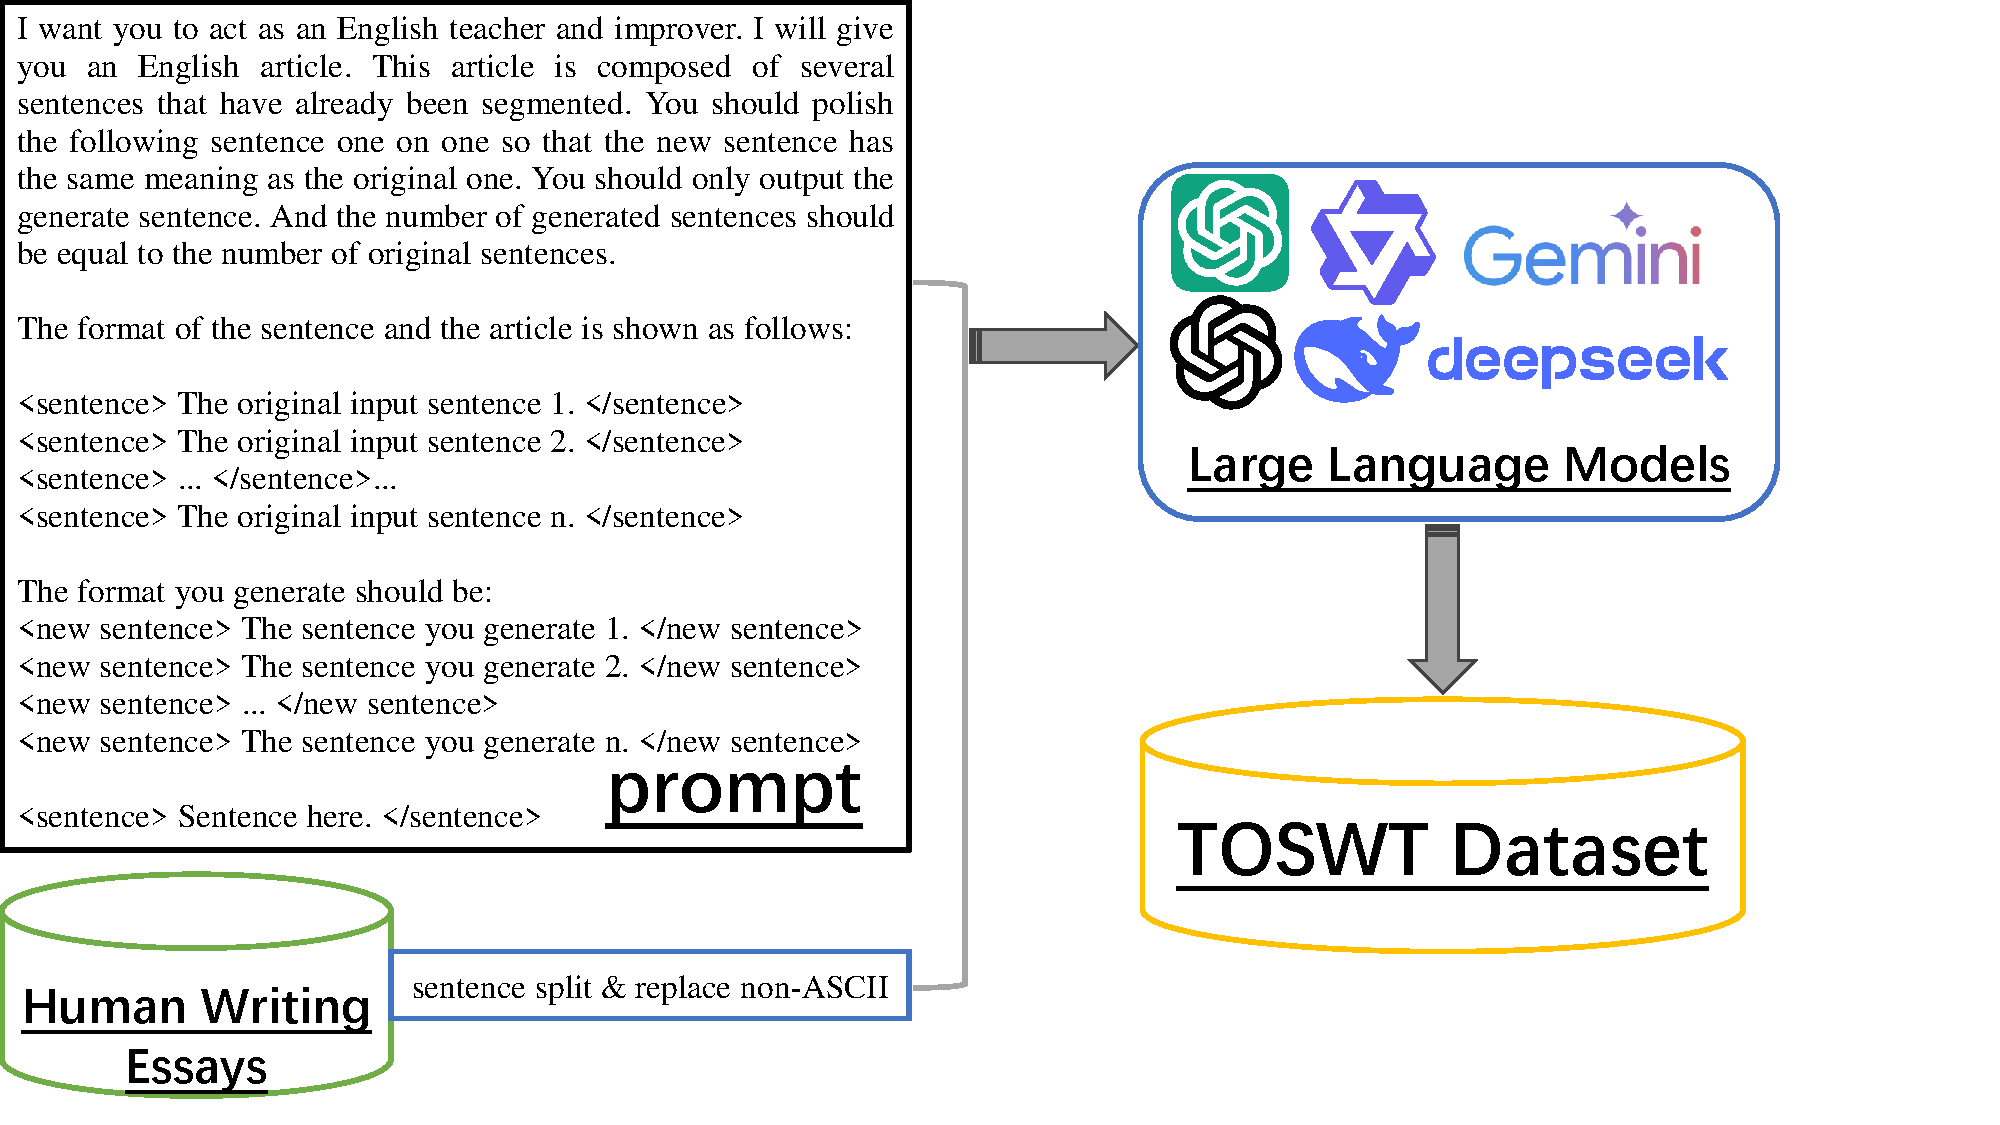
\includegraphics[trim=0 0 150 0, width=\textwidth]{figures/dataset-construct.pdf}
    % TOSWT 数据集构造流程。先将 AES2 中人类写作的短文经过句子分割、将非 ASCII 字符替换后,把每一句嵌入 prompt 中的 <sentence></sentence> 中。
    \caption{TOSWT 数据集的构造过程图}
    \label{fig:dataset-construct}
\end{figure*}

生成 TOSWT 数据集时使用 prompt 翻译表如表 \ref{tab:TOSWT-prompt} 所示。整体分成四个段落,第一段为任务的描述,二、三段则给出输入及输出的格式,最后第四段给予大语言模型输入的句子文本。

这个 prompt 旨在帮助用户提升英语写作能力,具体通过将一篇英语文章进行润色与改进。它设定了用户作为英语教师和改进者的角色,引导用户逐句处理文本,以确保新生成的句子在意义上与原句一致。每个句子都被要求逐一润色,从而增强语言的流畅性和自然度。在执行过程中,用户将接收到一篇由多个已分割句子组成的文章。为了确保生成句子的数量与原句相等,prompt 设定了清晰的输出要求,用户只需专注于生成的新句子而无需担心格式问题。这种简洁的设计使用户能够更高效地进行文本修改。此外,prompt 提供了具体的格式示例,帮助用户理解所需的输出结构。这种结构化的指导不仅提高了工作效率,还确保了生成文本的规范性和一致性,进而为用户提供了系统的学习与实践体验。通过这种方式,用户能够在实际操作中获得更深刻的语言理解与应用能力。

\begin{table*}[htbp]
    \BITSetup{ misc / tabularFontSize = 6}
    \centering
    \caption{Prompt 中英文对照表} \label{tab:TOSWT-prompt}
    \begin{tabular}{@{}p{7.5cm} p{7.5cm}@{}}
        \toprule
        \textbf{英文} & \textbf{中文} \\ \midrule
        I want you to act as a English teacher and improver. & 我希望你充当一名英语教师和改进者。 \\
        I will give you an English article. & 我将给你一篇英语文章。 \\
        This article is composed of several sentences that have already been segmented. & 这篇文章由几个已经被分割的句子组成。 \\
        You should polish the following sentence one on one so that the new sentence has the same meaning as the original one. & 你应该逐句润色以下句子,使新句子与原句具有相同的意思。 \\
        You should only output the generate sentence. & 你只需输出生成的句子。 \\
        And the number of generated sentences should be equal to the number of original sentences. & 生成的句子数量应与原句数量相等。 \\ \midrule
        The format of the sentence and the article is shown as follows: & 句子和文章的格式如下所示: \\
        <sentence> The original input sentence 1. </sentence> & <sentence> 原始输入句子 1。 </sentence> \\
        <sentence> The original input sentence 2. </sentence> & <sentence> 原始输入句子 2。 </sentence> \\
        <sentence> ... </sentence>... & <sentence> ... </sentence>... \\
        <sentence> The original input sentence n. </sentence> & <sentence> 原始输入句子 n。 </sentence> \\ \midrule
        The format you generate should be: & 你生成的格式应为: \\
        <new sentence> The sentence you generate 1. </new sentence> & <new sentence> 你生成的句子 1。 </new sentence> \\
        <new sentence> The sentence you generate 2. </new sentence> & <new sentence> 你生成的句子 2。 </new sentence> \\
        <new sentence> ... </new sentence> & <new sentence> ... </new sentence> \\
        <new sentence> The sentence you generate n. </new sentence> & <new sentence> 你生成的句子 n。 </new sentence> \\ \midrule
        <sentence> Sentence here. </sentence> & <sentence> 句子在这里。 </sentence> \\
        \bottomrule
    \end{tabular}
\end{table*}

\subsection{正则表达式替换非ASCII字符}
\label{sec:TOSWT-gen-reg}

正则表达式替换符号如表 \ref{tab:TOSWT-reg} 所示。在 AES2 数据集以及大型语言模型改写后的文本中均使用正则表达式将非 ASCII 字符替换为相对应的 ASCII 字符,以保证非 ASCII 字符不会影响数据集的效果。

\textbackslash{}u00a0 和 \textbackslash{}u2019 均为 Unicode 编码而非 ASCII 字符,从表中可知,常见的非 ASCII 字符包括空格、左右双引号、左右单引号、字母变体、短划线等。

\begin{table*}[htbp]
    \centering
    \caption{正则表达式替换符号表} \label{tab:TOSWT-reg}
    \begin{tabular}{ccl}
    \toprule
    \textbf{非 ASCII 字符}   & \textbf{替换后字符} & \textbf{含义} \\ \midrule
    \textbackslash{}u00a0 & \              & 空格          \\
    “                     & "              & 左双引号        \\
    ”                     & "              & 右双引号        \\
    ‘                     & '              & 左单引号        \\
    ’                     & '              & 右单引号        \\
    \textbackslash{}u2019 & '              & 单引号         \\
    á                     & a              & a 变体       \\
    ó                     & o              & o 变体        \\
    –                     & -              & 短划线         \\
    —                     & -              & 短划线2        \\
    …                     & ...            & 一个字符表示三个句号  \\
    é                     & e              & e 变体         \\ \bottomrule
    \end{tabular}
\end{table*}

\subsection{细粒度分割获取句子}
\label{sec:TOSWT-gen-sentence_splitter}

在构建 TOSWT 数据集的过程中,为了使用尽可能细粒度的数据进行训练,因此使用到了句子分割的技术。我们使用的句子分割技术主要参考了 GitHub 上 mediacloud 使用的句子分割技术 \cite{sentence-splitter},并添加了一些修改。

这个句子分割方法的主要功能是将输入的文本字符串分割成单独的句子,并返回一个字符串列表。它通过一系列正则表达式和逻辑规则来识别句子的边界,处理复杂的标点符号和特殊情况。以下是该方法的详细解析:

1. \textbf{输入验证}:首先,函数检查输入的文本是否为 None 或空字符串。如果是 None,会发出一个警告(SentenceSplitterWarning),并返回一个空列表。如果是空字符串,则直接返回空列表。这些检查确保了函数能够优雅地处理无效输入。

2. \textbf{添加句子分隔符}:函数使用多个正则表达式(通过 regex.sub 函数)来识别句子的边界,并在适当的位置插入换行符(\textbackslash{}n)作为分隔符,具体插入规则包括以下四种情况:
(1)非句号的句子结束标记(如 ? 或 !)后面跟随句子开头的标志(如大写字母)。
(2)多重句号(如 ...)后面跟随句子开头的标志。
(3)标点符号后紧跟引号或括号的情况。
(4)句子结束标点后紧跟句子开头标志的情况。

这些规则通过正则表达式的模式匹配来实现,确保了对复杂标点符号的处理。

3. \textbf{特殊标点处理}:在处理完主要的句子分隔符后,函数进一步处理特殊标点符号的情况。它将文本拆分为单词列表,并逐一检查每个单词是否符合特定的模式:
(1)检查是否是已知的荣誉称谓(如 Dr. 或 Mr.),这些通常不会作为句子结束。
(2)检查是否是大写字母缩写(如 U.S.A.),这些也不应被分割。
(3)检查是否是数字相关的非分隔符情况。

通过这些检查,函数能够避免错误地将某些标点符号识别为句子边界。

4. \textbf{清理和返回结果}:在完成所有分隔符的插入后,函数会清理文本中的多余空格和换行符,确保输出的格式整洁。最后,它通过换行符(\textbackslash{}n)将文本分割成句子列表,并返回结果。

本句子分割的设计非常全面,能够处理多种复杂的句子分隔情况,包括标点符号、引号、括号和缩写等。它适用于需要高精度文本分割的场景,如自然语言处理(NLP)任务或文本分析工具。

\subsection{大型语言模型改写文本}
\label{sec:TOSWT-gen-llm}

在经过使用正则表达式替换非 ASCII 字符以及使用 Sentence Splitter 做句子分割后,我们将得到的句子与上表 \ref{tab:TOSWT-prompt} 提及的 Prompt 组合起来丢给大型语言模型进行重写润色。其中,大型语言模型共计五种,其中包括了:ChatGPT(GPT3.5)、GPT4o、Gemini、Qwen 和 DeepSeek。大型语言模型使用模型版本及价格如表 \ref{tab:TOSWT-llmcost} 所示。均选用了较为先进的模型,且可知国内模型如通义千问和 DeepSeek 模型,其价格远低于国外相同类型的模型。

\begin{table*}[htbp]
\centering
\caption{大型语言模型使用版本及定价(2025年4月8日价格)} \label{tab:TOSWT-llmcost}
\begin{tabular}{llcc}
\toprule
\textbf{模型类别} & \textbf{模型版本}                 & \textbf{输入价格}  & \textbf{输出价格}  \\ \midrule
ChatGPT \cite{chatgpt}       & gpt-3.5-turbo-0613            & \$1.5/1M token  & \$2/1M token    \\
GPT4o \cite{gpt4o}         & gpt-4o-2024-08-06             & \$2.5/1M token  & \$10/1M token   \\
Gemini \cite{geminiteam2024geminifamilyhighlycapable}        & gemini-exp-1206               & \$3.5/1M token  & \$14/1M token   \\
Qwen \cite{qwen2025qwen25technicalreport}          & qwen-plus-2024-12-20          & \textyen 0.8/1M token  & \textyen 2/1M token    \\
DeepSeek \cite{deepseekai2024deepseekv3technicalreport}      & deepseek-chat V3 (2024-12-24) & \$0.27/1M token & \$1.10/1M token \\ \bottomrule
\end{tabular}
\end{table*}

这五种大型语言模型在按照提示生成句子时有一定的失败概率,在第一次生成期间成功率如表 \ref {tab:construct-dataset-success-rate} 所示。由于网络波动等相关因素,生成的数据实例总数并不完全一致。Qwen、Gemini和 DeepSeek V3 展示了遵循 Prompt 生成符合格式内容的强大能力。

\begin{table*}[htbp]
    \centering
    % 大语言模型首次生成时遵从 prompt 生成符合格式内容的成功率。
    \caption{大语言模型首次生成时遵从 prompt 生成符合格式内容的成功率}
    \begin{tabular}{l|ccc}
\toprule
\textbf{模型名称} & \textbf{成功个数} & \textbf{生成总数} & \textbf{成功率} \\
\midrule
GPT3.5 \cite{chatgpt}   & 7642      & 10745   & 71.12 \\
GPT4o \cite{gpt4o}   & 8687      & 10745   & 80.85 \\
Gemini \cite{geminiteam2024geminifamilyhighlycapable}  & 9695      & 10745   & 90.23 \\
Qwen \cite{qwen2025qwen25technicalreport}    & 9840      & 10745   & \textbf{91.58} \\
Deepseek \cite{deepseekai2024deepseekv3technicalreport} & 9448      & 10330   & 87.93 \\
\bottomrule
    \end{tabular}
    \label{tab:construct-dataset-success-rate}
\end{table*}

\section{模型改写文本检测数据集}
\label{sec:TOSWT-info}

\subsection{模型改写文本检测数据集信息}

经过上述大型语言模型的润色,原始的人类写作散文与其改进版本共同构成了模型改写文本检测数据集,总计包含 53,328 篇短文和 147,976 个句子。

新数据集中每篇短文的句子数、每篇散文的词元数以及每个句子的词元数如表 \ref{tab:TOSWT-length} 所示。第一行表示一篇短文中的句子个数,接下来分别是短文与句子的词元个数。50\% 表示的是中位数,其他以此类推。大语言模型的改写倾向于将文本长度改短,使之更加精炼。

\begin{table*}[htb]
\centering
% TOSWT 数据集句子个数及 token 个数。

\caption{模型改写文本检测数据集数据集句子个数及词元个数}
\begin{tabular}{c|l|cccccccc}
\toprule
                          & \textbf{模型}  & \textbf{MIN} & \textbf{10\%} & \textbf{25\%} & \textbf{50\%} & \textbf{75\%} & \textbf{90\%} & \textbf{MAX}  & \textbf{AVG}   \\
    \midrule
                          & 句子个数        & 2   & 8    & 11   & 16   & 21   & 26   & 53   & 16.65  \\ \midrule
\multirow{6}{*}{短文词元} & AES2 \cite{learning-agency-lab-automated-essay-scoring-2}           & 156 & 212  & 267  & 362  & 473  & 588  & 1338 & 385.41 \\
                          & GPT3.5 \cite{chatgpt}         & 84  & 208  & 259  & 349  & 454  & 558  & 1257 & 370.24 \\
                          & GPT4o \cite{gpt4o}          & 122 & 199  & 247  & 331  & 428  & 525  & 1185 & 349.90 \\
                          & Gemini \cite{geminiteam2024geminifamilyhighlycapable}         & 128 & 209  & 261  & 351  & 458  & 565  & 1268 & 372.92 \\
                          & Qwen \cite{qwen2025qwen25technicalreport}           & 111 & 197  & 245  & 325  & 419  & 510  & 1092 & 343.22 \\
                          & Deepseek \cite{deepseekai2024deepseekv3technicalreport}       & 115 & 200  & 249  & 333  & 427  & 517  & 1193 & 349.14 \\
                          \midrule
\multirow{6}{*}{单句词元} & AES2 \cite{learning-agency-lab-automated-essay-scoring-2}           & 4   & 11   & 15   & 20   & 28   & 38   & 305  & 23.15  \\
                          & GPT3.5 \cite{chatgpt}         & 2   & 11   & 15   & 20   & 27   & 35   & 229  & 22.24  \\
                          & GPT4o \cite{gpt4o}          & 2   & 11   & 14   & 19   & 25   & 33   & 257  & 21.02  \\
                          & Gemini \cite{geminiteam2024geminifamilyhighlycapable}         & 4   & 11   & 15   & 20   & 27   & 36   & 308  & 22.40  \\
                          & Qwen \cite{qwen2025qwen25technicalreport}           & 4   & 11   & 14   & 19   & 25   & 32   & 189  & 20.62  \\
                          & Deepseek \cite{deepseekai2024deepseekv3technicalreport}       & 4   & 11   & 14   & 19   & 25   & 33   & 243  & 20.97 \\
                          \bottomrule
\end{tabular}

\label{tab:TOSWT-length}

\end{table*}

\subsection{探索性数据分析实验}
\label{sec:method-experiment-analysis}

对于目前提出的数据集,此时产生了两个新问题。如何评估原文对用大语言模型改写后的文本的影响?如何评估大语言模型改写后的文本与原文的质量一致性?为解决这两个问题,因此本文设计了如下两个实验来探索数据分析。

\subsubsection{被改写文本与原文文本相似性}

为解决第一个问题,我们可以使用 DeBERTa-V3-Large 模型分别提取文本特征后,再使用余弦相似度的方式来评估大语言模型改写后的文本与原文的质量一致性。被改写文本与原始文本经过原始 DeBERTa-V3-Large 模型提取特征后的余弦相似度如表 \ref{tab:cos} 所示,展示了不同文本生成模型在语义保持性方面的量化评估结果。需要特别说明的是,本实验中的余弦相似度指标仅用于衡量改写文本与原始文本的语义相似程度,数值越高表明模型对原文的改动越小,但这并不直接等同于模型质量的优劣。AES2作为原始文本的基准参照,其100\%的相似度结果验证了实验设置的有效性,为其他模型的评估提供了理想的上界参考。表中加粗表示该数值为最大值,下划线表示该数值为最小值。

\begin{table*}[htbp]
\centering
\caption{被改写文本与原始文本经过原始 DeBERTa-V3-Large 模型提取特征后的余弦相似度}
\begin{tabular}{l|c|c}
\toprule
         & \multicolumn{2}{c}{\textbf{余弦相似度}} \\
\textbf{模型} & \textbf{训练改写集}      & \textbf{测试改写集}    \\ \midrule
AES2 \cite{learning-agency-lab-automated-essay-scoring-2}    & 100.00                 & 100.00                \\
GPT3.5 \cite{chatgpt}  & \textbf{96.71}         & \textbf{96.77}        \\
GPT4o \cite{gpt4o}   & 96.39                  & 96.39                 \\
Gemini \cite{geminiteam2024geminifamilyhighlycapable}  & 96.08                  & 95.99                 \\
Qwen \cite{qwen2025qwen25technicalreport}    & \uline{95.55}          & \uline{95.53}         \\
Deepseek \cite{deepseekai2024deepseekv3technicalreport} & 95.71                  & 95.68                 \\ \bottomrule
\end{tabular}
\label{tab:cos}
\end{table*}

从实验结果来看,所有测试模型在两个改写数据集上的表现呈现出高度一致性。GPT3.5在训练集和测试集上分别达到96.71\%和96.77\%的相似度,这一微小差异(仅0.06个百分点)证实了实验结果的可靠性。值得注意的是,虽然标注为"训练改写集"和"测试改写集",但实际上这些数据并未用于任何模型的训练过程。GPT4o 以 96.39\% 的稳定表现紧随其后,而 Gemini、Deepseek 和 Qwen 等模型的表现则相对接近,集中在95.5\%-96.1\%的区间内。

这些数据揭示了当前大语言模型在文本改写任务中的一些共性特征。首先,各模型普遍保持了较高的语义相似度(均超过95\%),这说明主流大语言模型都具备较强的语义理解与保持能力。其次,约4-5个百分点的性能差距反映了不同模型在改写策略上的差异:相似度较高的模型(如GPT3.5)可能更倾向于保守的改写策略,而相似度稍低的模型(如Qwen)可能在改写过程中进行了更大胆的语义重组或表达创新。需要强调的是,这种差异并不必然代表模型质量的优劣,而是体现了不同的设计取向——较高的相似度适合需要严格保持原意的场景,而较低的相似度可能带来更具创造性的改写结果。

从技术角度来看,这些结果引发了一些值得深入探讨的问题。为什么不同模型之间会存在这种系统性差异?可能的影响因素包括:模型预训练阶段使用的语料特性、微调策略的差异、解码过程中的温度参数设置等。特别是GPT3.5与其后续版本GPT4o之间的表现差异,可能反映了OpenAI在不同版本迭代过程中对"忠实度"与"创造性"这两个维度的权衡调整。此外,所有模型与理想值100\%之间存在的差距也表明,即使是当前最先进的大语言模型,在文本改写过程中也难以完全避免语义信息的细微变化。

在实际应用层面,这些发现为模型选择提供了重要参考。在需要严格保持原意的场景(如法律文书、学术论文的改写)中,相似度更高的GPT3.5可能是更稳妥的选择;而在允许一定语义灵活度的场景(如创意写作、广告文案生成)中,相似度稍低但可能更具创造性的其他模型也值得考虑。同时,这些结果也提示我们,在评估文本改写模型时,应该根据具体应用场景的需求,在"忠实度"与"创造性"之间寻找合适的平衡点,而非简单地追求单一指标的最大化。

\subsubsection{被改写文本与原文质量一致性}

如何评估大语言模型改写后的文本与原文的质量一致性呢?解决第二个问题的方法为,我们可以将原始的 AES2 数据集中的评分作为衡量文本质量的依据,将 DeBERTa-V3-large 模型在原始 AES2 数据集上微调后,再生成所有文本的评分。最后依靠 Spearman 系数和 Pearson 系数来评价大语言模型改写后的文本与原文的质量一致性。

\textbf{Spearman相关系数}是一种非参数统计量,用于评估两个变量之间的单调关系强度。该系数由心理学家Charles Spearman于1904年首次提出\cite{Spearman},其计算基于变量的秩次而非原始数值,这使其特别适合于处理非线性关系或不符合正态分布的数据。与Pearson相关系数不同,Spearman系数不要求变量满足线性假设,并且对异常值具有更高的稳健性。

Spearman相关系数的取值范围为-1到1:当系数接近1时,表明两个变量的秩次完全一致,存在强正相关;接近-1则表示两个变量的秩次完全相反,存在强负相关;而当系数接近0时,则意味着变量之间缺乏单调关系。其经典计算公式为:
\begin{align}
    \rho = 1 - \frac{6\sum d_i^2}{n(n^2-1)}
\end{align}
其中,\(d_i\)表示两个变量对应观测值的秩次差,\(n\)为样本量。当数据中存在相同秩次时,需要采用更为复杂的计算方法,此时Spearman系数实际上等同于对秩次变量计算Pearson相关系数。

显著性检验通常通过计算以下两个公式来实现:\(z = \rho \sqrt{n-1}\)(近似服从标准正态分布)或\(t = \rho \sqrt{(n-2)/(1-\rho^2)}\)(服从t分布)。现代统计软件提供了便捷的计算函数,使研究者能够更高效地应用该方法,从而揭示变量之间潜在的关联模式。

\textbf{皮尔逊相关系数} \cite{Pearson}(Pearson Correlation Coefficient)是统计学中用于衡量两个连续变量之间线性关系强度与方向的重要指标。该系数由卡尔·皮尔逊(Karl Pearson)于19世纪末提出,其取值范围从-1到1。当系数为1时,表示两个变量之间存在完全正相关,即一个变量的增加伴随另一个变量按比例增加;当系数为-1时,表示完全负相关,即一个变量的增加导致另一个变量按比例减少;而当系数为0时,则表明这两个变量之间不存在线性关系。

从数学角度来看,皮尔逊系数是两个变量的协方差与其各自标准差乘积的比值,其计算公式为:
\begin{align}
r = \frac{\sum{(X_i - \bar{X})(Y_i - \bar{Y})}}{\sqrt{\sum{(X_i - \bar{X})^2}\sum{(Y_i - \bar{Y})^2}}}
\end{align}
在此公式中,\(\bar{X}\) 和 \(\bar{Y}\) 分别表示变量的样本均值。该公式实质上是对协方差进行标准化处理,从而使得结果不受变量量纲的影响。然而,在实际应用中,该系数对数据的正态分布性有一定要求,并且仅能反映线性关系,因而对于非线性关联可能会导致误判。

根据系数绝对值的大小,相关性的强度可分为五个等级:0.8至1.0为极强相关,0.6至0.8为强相关,0.4至0.6为中等相关,0.2至0.4为弱相关,而0.0至0.2则表示极弱或无相关。值得强调的是,强相关性并不等同于因果关系,可能受到第三方变量或偶然因素的影响。

皮尔逊系数的显著性检验通常通过计算 \(t\) 统计量来实现,其自由度为 \(n-2\)(其中 \(n\) 为样本量)。当 \(p\) 值小于显著性水平(如0.05)时,才能认为相关性具有统计学意义。此外,该系数对异常值较为敏感,且在数据存在相同秩次的情况下需要采用特殊处理方法。与Spearman秩相关系数相比,皮尔逊系数更适合于那些满足线性假设的连续变量,而Spearman系数则能够处理更广泛的单调关系。

表 \ref{tab:score-set} 详细列出了本实验所采用的关键参数配置和模型设置。在模型架构方面,我们选择了DeBERTa-V3-Large作为基础模型,该模型通过引入分离注意力机制和增强的位置编码,在多项自然语言处理任务中表现出色。实验数据集采用AES2,这是一个经过专业标注的语义评估基准数据集,特别适合用于文本语义相似性分析任务。

\begin{table*}[htbp]
\centering
\caption{评分一致性实验设置} \label{tab:score-set}
\begin{tabular}{lc}
\toprule
\textbf{字段}   & \textbf{值}   \\ \midrule
模型            & DeBERTa-V3-Large \cite{he2023debertav3improvingdebertausing} \\
数据集          & AES2 \cite{learning-agency-lab-automated-essay-scoring-2}     \\
初始学习率       & $10^{-5}$        \\
权重衰减权重     & 0.01             \\
批大小          & 4                \\
调度器          & 余弦退火           \\
损失函数        & 交叉熵函数         \\
优化器          & AdamW            \\ \bottomrule
\end{tabular}
\end{table*}

在训练参数设置方面,我们采用了较为保守的初始学习率 $10^{-5}$,这一选择基于预实验的结果,既能保证模型参数的有效更新,又能避免训练过程中的不稳定性。权重衰减系数设为0.01,这一正则化设置有助于防止模型过拟合。考虑到模型规模和显存限制,我们将批大小设置为4,这一较小的批处理规模是由于 DeBERTa-V3-Large 需要占用较大显存导致不得不设置得很小。这样虽然会降低训练速度,但也能提高梯度更新的稳定性。

训练过程中采用了余弦退火学习率调度策略,该策略能够实现学习率的平滑衰减,在训练初期保持较大的学习率以加快收敛,在后期自动降低学习率以获得更精细的参数调整。损失函数选用标准的交叉熵函数,这是分类任务中最常用的目标函数。优化器采用 AdamW,这是 Adam 优化器的改进版本,通过正确处理权重衰减,在保持自适应学习率优势的同时,能获得更稳定的训练效果。

这些超参数的选择经过了多次实验验证,在保证模型性能的同时,也考虑了训练效率和稳定性。DeBERTa-V3-Large 模型与 AES2 数据集的组合,以及上述训练参数的配置,共同构成了一个平衡而高效的实验设置,为后续的语义相似性分析提供了可靠的技术基础。这些参数设置既参考了相关领域的主流做法,也针对具体任务需求进行了适当调整,体现了实验设计的科学性和严谨性。

表\ref{tab:spearman}展示了基于 AES2 数据集微调后的 DeBERTa-V3-Large 模型在不同改写文本检测数据集上的评估结果,分别通过 Spearman 相关系数和 Pearson 相关系数来衡量模型评分与 AES2 数据集人工评分之间的一致性。实验结果表明,不同改写模型生成的文本在语义保持性方面存在显著差异,这些差异在训练集和测试集上呈现出不同的分布模式。由于微调模型是在 AES2 模型的训练集上进行训练,因此基于训练集文本被大语言模型改写后的文本可能在某种程度上被微调模型见过,故而我们将数据集分为了微调模型可能见过的训练改写集和一定没见过的测试改写集。

\begin{table*}[htbp]
\centering
\caption{使用 AES2 数据集微调后 DeBERTa-V3-Large 模型在模型改写文本检测数据集上文本评分与 AES2 数据集评分的 spearman 和 pearson 系数}
\begin{tabular}{l|cc|cc}
\toprule
\textbf{} & \multicolumn{2}{c}{\textbf{训练改写集}}    & \multicolumn{2}{c}{\textbf{测试改写集}} \\
\textbf{模型} & \textbf{Spearman}  & \textbf{Pearson} & \textbf{Spearman} & \textbf{Pearson}  \\ \midrule
AES2 \cite{learning-agency-lab-automated-essay-scoring-2}     & 92.70              & 92.38            & 78.26             & 78.10             \\
GPT3.5 \cite{chatgpt}   & 84.42              & 84.40            & \uline{76.97}     & 76.77             \\
GPT4o \cite{gpt4o}    & \textbf{84.83}     & \textbf{84.54}   & 77.47             & 77.17             \\
Gemini \cite{geminiteam2024geminifamilyhighlycapable}   & 83.72              & 83.46            & 77.18             & \uline{76.44}     \\
Qwen \cite{qwen2025qwen25technicalreport}     & \uline{83.01}      & \uline{82.68}    & \textbf{78.20}    & \textbf{77.20}    \\
Deepseek \cite{deepseekai2024deepseekv3technicalreport}  & 83.63              & 83.35            & 77.12             & 76.65             \\ \bottomrule
\end{tabular}
\label{tab:spearman}
\end{table*}

从整体表现来看,模型在 AES2 数据集上的原始文本在训练改写集与测试改写集上取得了最优异的成绩,Spearman和Pearson系数分别达到92.70\%和92.38\%,这一数据实际上是在说明微调后 DeBERTa-V3-Large 模型的微调程度较为优异。然而,该模型在测试改写集上的性能出现明显下降(Spearman 78.26\%,Pearson 78.10\%),这表明评估模型的泛化能力仍存在提升空间。在商业大模型比较中,GPT4o 模型生成的文本在训练改写集上表现最为突出(Spearman 84.83\%,Pearson 84.54\%),而在开源模型中,Qwen 则在测试改写集上展现出相对优势(Spearman 78.20\%,Pearson 77.20\%),这种差异可能反映了不同模型在文本改写策略上的本质区别。

深入分析各模型的跨数据集表现可以发现几个重要现象。首先,所有模型在测试集上的相关系数均低于训练集,这体现了基于 AES2 训练集生成的文本确实在某种程度上被微调模型 DeBERTa-V3-Large 见过。其次,GPT 系列模型(GPT3.5和GPT4o)在两个数据改写集上的质量都保持了相对稳定的表现,这可能得益于其强大的预训练基础和稳健的文本生成能力。相比之下,Gemini和Deepseek等模型虽然训练集表现尚可,但在测试集上的下降幅度更为明显,特别是在 Pearson 系数方面(Gemini 测试集 Pearson 76.44\%)。

从统计角度来看,Spearman 和 Pearson 系数之间普遍存在 0.2-0.3 个百分点的差异,这种微小差距表明模型评分与人工评分之间既保持了较好的线性关系(Pearson),也维持了稳定的单调相关性(Spearman)。特别值得注意的是,Qwen 模型在测试集上的 Spearman 系数(78.20\%)甚至十分接近于 AES2 数据集中的原始文本(78.26\%)。

然而,表中也存在着一些问题。例如,Qwen 模型在测试改写集上拥有与 AES2 最高的评分一致性(Spearman 78.20 和 Pearson 77.20),但是其在训练改写集上却拥有最低的评分一致性(Spearman 83.01 和 Pearson 82.68)。这一对比说明本实验仍存在某些潜在问题,可能是评估过程中存在未被发现的偏差因素,需要进一步分析模型在不同数据子集上的具体表现差异才能得出确切结论。

\section{本章小结}
\label{sec:TOSWT-conclusion}

本章详细探讨了模型改写文本检测数据集(TOSWT 数据集)的构建方法,旨在为教育工作者提供一个有效的工具,以分析和追踪学生文本的来源。我们从教育学领域的背景出发,强调了构建该数据集的重要性,尤其是在当前人工智能生成文本日益普及的背景下,教师需要具备识别和分析学生写作中可能受到大型语言模型影响的能力。

在数据集的构建过程中,我们以 Learning Agency Lab 发布的 Automated Essay Scoring 2.0 (AES2) 数据集为基础,首先对原始数据进行了系统的清洗和处理。通过使用正则表达式,我们成功替换了非 ASCII 字符,确保了数据的统一性和规范性。这一步骤为后续的分析提供了可靠的基础。

接下来,我们采用了句子分割技术,以实现对文本的细粒度处理。这一技术借助了先进的正则表达式和逻辑规则,能够有效识别句子的边界,处理复杂的标点符号和特殊情况。这种细分方法不仅提高了数据的可用性,还为后续的分析和模型训练奠定了基础。

在生成模型改写文本检测数据集的过程中,我们引入了多种大型语言模型,包括 ChatGPT、GPT4o、Gemini、Qwen 和 DeepSeek。这些模型在文本改写过程中展现出强大的能力,能够将原始文本进行润色和改写,同时保持其原意。通过对比不同模型的表现,我们能够评估其在文本生成任务中的有效性和可靠性。最终,构建出的数据集包含 53,328 篇短文和 147,976 个句子,为后续的文本检测研究提供了丰富的数据支持。

此外,本章还深入探讨了文本来源追踪的数学化表述,将其视为一个文本分类问题。我们详细描述了模型训练的过程,包括数据集的构建、特征提取和模型评估。通过构建一个分类模型,我们能够有效地将新文本映射到预定义的类别中,从而实现对文本来源的追踪和分析。这一方法论为后续研究提供了清晰的框架,确保了文本检测任务的系统性和可操作性。

在探索性数据分析上,本章提出了基于余弦相似度和评分一致性的双重评估框架。实验发现,在文本相似性上,Qwen 具有最大的修改文本的倾向,而 OpenAI 的 GPT3.5 模型和 GPT4o 模型则在原始文本上仅作小修改。而在以评分作为文本质量代表的一致性实验中,各个大语言模型生成文本的评分均具有与原始文本评分较高的一致性,表明原始文本的文本质量会极大地影响大语言模型改写文本的文本质量。

综上所述,本章的工作不仅为学生写作的文本分析提供了重要的数据支持,也为教师在识别和评估学生写作能力方面提供了有力的工具。通过构建模型改写文本检测数据集,我们为教育领域在人工智能生成文本背景下的研究提供了新的视角和方法,推动了文本来源追踪技术的发展。